\batchmode
\documentclass[twoside]{book}

% Packages required by doxygen
\usepackage{fixltx2e}
\usepackage{calc}
\usepackage{doxygen}
\usepackage[export]{adjustbox} % also loads graphicx
\usepackage{graphicx}
\usepackage[utf8]{inputenc}
\usepackage{makeidx}
\usepackage{multicol}
\usepackage{multirow}
\PassOptionsToPackage{warn}{textcomp}
\usepackage{textcomp}
\usepackage[nointegrals]{wasysym}
\usepackage[table]{xcolor}

% Font selection
\usepackage[T1]{fontenc}
\usepackage[scaled=.90]{helvet}
\usepackage{courier}
\usepackage{amssymb}
\usepackage{sectsty}
\renewcommand{\familydefault}{\sfdefault}
\allsectionsfont{%
  \fontseries{bc}\selectfont%
  \color{darkgray}%
}
\renewcommand{\DoxyLabelFont}{%
  \fontseries{bc}\selectfont%
  \color{darkgray}%
}
\newcommand{\+}{\discretionary{\mbox{\scriptsize$\hookleftarrow$}}{}{}}

% Page & text layout
\usepackage{geometry}
\geometry{%
  a4paper,%
  top=2.5cm,%
  bottom=2.5cm,%
  left=2.5cm,%
  right=2.5cm%
}
\tolerance=750
\hfuzz=15pt
\hbadness=750
\setlength{\emergencystretch}{15pt}
\setlength{\parindent}{0cm}
\setlength{\parskip}{3ex plus 2ex minus 2ex}
\makeatletter
\renewcommand{\paragraph}{%
  \@startsection{paragraph}{4}{0ex}{-1.0ex}{1.0ex}{%
    \normalfont\normalsize\bfseries\SS@parafont%
  }%
}
\renewcommand{\subparagraph}{%
  \@startsection{subparagraph}{5}{0ex}{-1.0ex}{1.0ex}{%
    \normalfont\normalsize\bfseries\SS@subparafont%
  }%
}
\makeatother

% Headers & footers
\usepackage{fancyhdr}
\pagestyle{fancyplain}
\fancyhead[LE]{\fancyplain{}{\bfseries\thepage}}
\fancyhead[CE]{\fancyplain{}{}}
\fancyhead[RE]{\fancyplain{}{\bfseries\leftmark}}
\fancyhead[LO]{\fancyplain{}{\bfseries\rightmark}}
\fancyhead[CO]{\fancyplain{}{}}
\fancyhead[RO]{\fancyplain{}{\bfseries\thepage}}
\fancyfoot[LE]{\fancyplain{}{}}
\fancyfoot[CE]{\fancyplain{}{}}
\fancyfoot[RE]{\fancyplain{}{\bfseries\scriptsize Generated by Doxygen }}
\fancyfoot[LO]{\fancyplain{}{\bfseries\scriptsize Generated by Doxygen }}
\fancyfoot[CO]{\fancyplain{}{}}
\fancyfoot[RO]{\fancyplain{}{}}
\renewcommand{\footrulewidth}{0.4pt}
\renewcommand{\chaptermark}[1]{%
  \markboth{#1}{}%
}
\renewcommand{\sectionmark}[1]{%
  \markright{\thesection\ #1}%
}

% Indices & bibliography
\usepackage{natbib}
\usepackage[titles]{tocloft}
\setcounter{tocdepth}{3}
\setcounter{secnumdepth}{5}
\makeindex

% Hyperlinks (required, but should be loaded last)
\usepackage{ifpdf}
\ifpdf
  \usepackage[pdftex,pagebackref=true]{hyperref}
\else
  \usepackage[ps2pdf,pagebackref=true]{hyperref}
\fi
\hypersetup{%
  colorlinks=true,%
  linkcolor=blue,%
  citecolor=blue,%
  unicode%
}

% Custom commands
\newcommand{\clearemptydoublepage}{%
  \newpage{\pagestyle{empty}\cleardoublepage}%
}

\usepackage{caption}
\captionsetup{labelsep=space,justification=centering,font={bf},singlelinecheck=off,skip=4pt,position=top}

%===== C O N T E N T S =====

\begin{document}

% Titlepage & ToC
\hypersetup{pageanchor=false,
             bookmarksnumbered=true,
             pdfencoding=unicode
            }
\pagenumbering{alph}
\pagenumbering{arabic}
\hypersetup{pageanchor=true}

%--- Begin generated contents ---
\chapter{Example problem\+: Adaptive solution of the 2D Poisson equation with flux boundary conditions}
\label{index}\hypertarget{index}{}\hypertarget{index_q}{}\section{A few quick questions...}\label{index_q}
Since {\ttfamily oomph-\/lib} is developed as open-\/source software, any evidence that the code is being downloaded and used is very helpful for us as it helps to justify our continued work on this project.

We would therefore be extremely grateful if you could provide the information requested in the form below. Pressing the \char`\"{}submit\char`\"{} button will get you to the actual download page.

{\bfseries Note\+:} 
\begin{DoxyItemize}
\item All information will be treated as confidential. 
\item If you provide your email address and check the appropriate box we will add you to our mailing list to inform you of upgrades and bug fixes to the code. Rest assured that the mailing list is {\bfseries very low volume} -- we have better things to do than to bombard you with email. 
\item If you still feel reluctant to provide any of the information requested, feel free to enter some dummy input. The form will check that {\bfseries some} information has been entered but entering your name as \char`\"{}\+Joe Cool\char`\"{} is perfectly acceptable -- this is to discourage people from not providing the information simply because they are too lazy to type... 
\end{DoxyItemize}



 







 

 \hypertarget{index_pdf}{}\section{P\+D\+F file}\label{index_pdf}
A \href{../latex/refman.pdf}{\tt pdf version} of this document is available. \end{document}

\chapter{Namespace Index}
\section{Namespace List}
Here is a list of all namespaces with brief descriptions\+:\begin{DoxyCompactList}
\item\contentsline{section}{\hyperlink{namespaceGlobal__Physical__Variables}{Global\+\_\+\+Physical\+\_\+\+Variables} \\*Global variables that represent physical properties }{\pageref{namespaceGlobal__Physical__Variables}}{}
\item\contentsline{section}{\hyperlink{namespaceoomph}{oomph} }{\pageref{namespaceoomph}}{}
\item\contentsline{section}{\hyperlink{namespacePhysical__Variables}{Physical\+\_\+\+Variables} \\*Namespace for the solution of 2D linear shell equation }{\pageref{namespacePhysical__Variables}}{}
\end{DoxyCompactList}

\chapter{Hierarchical Index}
\section{Class Hierarchy}
This inheritance list is sorted roughly, but not completely, alphabetically\+:\begin{DoxyCompactList}
\item Problem\begin{DoxyCompactList}
\item \contentsline{section}{Unstructured\+Solid\+Problem$<$ E\+L\+E\+M\+E\+NT $>$}{\pageref{classUnstructuredSolidProblem}}{}
\end{DoxyCompactList}
\end{DoxyCompactList}

\chapter{Class Index}
\section{Class List}
Here are the classes, structs, unions and interfaces with brief descriptions\+:\begin{DoxyCompactList}
\item\contentsline{section}{\hyperlink{classPMLProblem}{P\+M\+L\+Problem$<$ E\+L\+E\+M\+E\+N\+T $>$} }{\pageref{classPMLProblem}}{}
\item\contentsline{section}{\hyperlink{classGlobalParameters_1_1TestPMLMapping}{Global\+Parameters\+::\+Test\+P\+M\+L\+Mapping} }{\pageref{classGlobalParameters_1_1TestPMLMapping}}{}
\end{DoxyCompactList}

\chapter{File Index}
\section{File List}
Here is a list of all files with brief descriptions\+:\begin{DoxyCompactList}
\item\contentsline{section}{\hyperlink{jeffery__orbit_8cc}{jeffery\+\_\+orbit.\+cc} }{\pageref{jeffery__orbit_8cc}}{}
\item\contentsline{section}{\hyperlink{jeffery__orbit_8txt__doxygenified_8h}{jeffery\+\_\+orbit.\+txt\+\_\+doxygenified.\+h} }{\pageref{jeffery__orbit_8txt__doxygenified_8h}}{}
\item\contentsline{section}{\hyperlink{my__taylor__hood__elements_8h}{my\+\_\+taylor\+\_\+hood\+\_\+elements.\+h} }{\pageref{my__taylor__hood__elements_8h}}{}
\end{DoxyCompactList}

\chapter{Namespace Documentation}
\hypertarget{namespaceTanhSolnForPoisson}{}\section{Tanh\+Soln\+For\+Poisson Namespace Reference}
\label{namespaceTanhSolnForPoisson}\index{Tanh\+Soln\+For\+Poisson@{Tanh\+Soln\+For\+Poisson}}


Namespace for exact solution for Poisson equation with sharp step.  


\subsection*{Functions}
\begin{DoxyCompactItemize}
\item 
void \hyperlink{namespaceTanhSolnForPoisson_af7896e9c18ce6438c73ae2a875e8b7de}{get\+\_\+exact\+\_\+u} (const Vector$<$ double $>$ \&x, Vector$<$ double $>$ \&u)
\begin{DoxyCompactList}\small\item\em Exact solution as a Vector. \end{DoxyCompactList}\item 
void \hyperlink{namespaceTanhSolnForPoisson_af197decab980d38d2037032780723984}{get\+\_\+exact\+\_\+u} (const Vector$<$ double $>$ \&x, double \&u)
\begin{DoxyCompactList}\small\item\em Exact solution as a scalar. \end{DoxyCompactList}\item 
void \hyperlink{namespaceTanhSolnForPoisson_ae1b9d6789ff301e3d63a4e292213036c}{get\+\_\+source} (const Vector$<$ double $>$ \&x, double \&source)
\begin{DoxyCompactList}\small\item\em Source function to make it an exact solution. \end{DoxyCompactList}\end{DoxyCompactItemize}
\subsection*{Variables}
\begin{DoxyCompactItemize}
\item 
double \hyperlink{namespaceTanhSolnForPoisson_ae676ccd186d5df119cce811596d949c1}{Alpha}
\begin{DoxyCompactList}\small\item\em Parameter for steepness of step. \end{DoxyCompactList}\item 
double \hyperlink{namespaceTanhSolnForPoisson_ae07364a1d73b28e5e250bda6c8954f01}{Beta}
\begin{DoxyCompactList}\small\item\em Parameter for angle of step. \end{DoxyCompactList}\end{DoxyCompactItemize}


\subsection{Detailed Description}
Namespace for exact solution for Poisson equation with sharp step. 

\subsection{Function Documentation}
\mbox{\Hypertarget{namespaceTanhSolnForPoisson_af7896e9c18ce6438c73ae2a875e8b7de}\label{namespaceTanhSolnForPoisson_af7896e9c18ce6438c73ae2a875e8b7de}} 
\index{Tanh\+Soln\+For\+Poisson@{Tanh\+Soln\+For\+Poisson}!get\+\_\+exact\+\_\+u@{get\+\_\+exact\+\_\+u}}
\index{get\+\_\+exact\+\_\+u@{get\+\_\+exact\+\_\+u}!Tanh\+Soln\+For\+Poisson@{Tanh\+Soln\+For\+Poisson}}
\subsubsection{\texorpdfstring{get\+\_\+exact\+\_\+u()}{get\_exact\_u()}\hspace{0.1cm}{\footnotesize\ttfamily [1/2]}}
{\footnotesize\ttfamily void Tanh\+Soln\+For\+Poisson\+::get\+\_\+exact\+\_\+u (\begin{DoxyParamCaption}\item[{const Vector$<$ double $>$ \&}]{x,  }\item[{Vector$<$ double $>$ \&}]{u }\end{DoxyParamCaption})}



Exact solution as a Vector. 



Definition at line 61 of file mesh\+\_\+from\+\_\+triangle\+\_\+poisson.\+cc.



Referenced by Poisson\+Problem$<$ E\+L\+E\+M\+E\+N\+T $>$\+::actions\+\_\+before\+\_\+newton\+\_\+solve(), and Poisson\+Problem$<$ E\+L\+E\+M\+E\+N\+T $>$\+::doc\+\_\+solution().

\mbox{\Hypertarget{namespaceTanhSolnForPoisson_af197decab980d38d2037032780723984}\label{namespaceTanhSolnForPoisson_af197decab980d38d2037032780723984}} 
\index{Tanh\+Soln\+For\+Poisson@{Tanh\+Soln\+For\+Poisson}!get\+\_\+exact\+\_\+u@{get\+\_\+exact\+\_\+u}}
\index{get\+\_\+exact\+\_\+u@{get\+\_\+exact\+\_\+u}!Tanh\+Soln\+For\+Poisson@{Tanh\+Soln\+For\+Poisson}}
\subsubsection{\texorpdfstring{get\+\_\+exact\+\_\+u()}{get\_exact\_u()}\hspace{0.1cm}{\footnotesize\ttfamily [2/2]}}
{\footnotesize\ttfamily void Tanh\+Soln\+For\+Poisson\+::get\+\_\+exact\+\_\+u (\begin{DoxyParamCaption}\item[{const Vector$<$ double $>$ \&}]{x,  }\item[{double \&}]{u }\end{DoxyParamCaption})}



Exact solution as a scalar. 



Definition at line 68 of file mesh\+\_\+from\+\_\+triangle\+\_\+poisson.\+cc.

\mbox{\Hypertarget{namespaceTanhSolnForPoisson_ae1b9d6789ff301e3d63a4e292213036c}\label{namespaceTanhSolnForPoisson_ae1b9d6789ff301e3d63a4e292213036c}} 
\index{Tanh\+Soln\+For\+Poisson@{Tanh\+Soln\+For\+Poisson}!get\+\_\+source@{get\+\_\+source}}
\index{get\+\_\+source@{get\+\_\+source}!Tanh\+Soln\+For\+Poisson@{Tanh\+Soln\+For\+Poisson}}
\subsubsection{\texorpdfstring{get\+\_\+source()}{get\_source()}}
{\footnotesize\ttfamily void Tanh\+Soln\+For\+Poisson\+::get\+\_\+source (\begin{DoxyParamCaption}\item[{const Vector$<$ double $>$ \&}]{x,  }\item[{double \&}]{source }\end{DoxyParamCaption})}



Source function to make it an exact solution. 



Definition at line 75 of file mesh\+\_\+from\+\_\+triangle\+\_\+poisson.\+cc.



Referenced by main().



\subsection{Variable Documentation}
\mbox{\Hypertarget{namespaceTanhSolnForPoisson_ae676ccd186d5df119cce811596d949c1}\label{namespaceTanhSolnForPoisson_ae676ccd186d5df119cce811596d949c1}} 
\index{Tanh\+Soln\+For\+Poisson@{Tanh\+Soln\+For\+Poisson}!Alpha@{Alpha}}
\index{Alpha@{Alpha}!Tanh\+Soln\+For\+Poisson@{Tanh\+Soln\+For\+Poisson}}
\subsubsection{\texorpdfstring{Alpha}{Alpha}}
{\footnotesize\ttfamily double Tanh\+Soln\+For\+Poisson\+::\+Alpha}



Parameter for steepness of step. 



Definition at line 54 of file mesh\+\_\+from\+\_\+triangle\+\_\+poisson.\+cc.



Referenced by Poisson\+Problem$<$ E\+L\+E\+M\+E\+N\+T $>$\+::\+Poisson\+Problem().

\mbox{\Hypertarget{namespaceTanhSolnForPoisson_ae07364a1d73b28e5e250bda6c8954f01}\label{namespaceTanhSolnForPoisson_ae07364a1d73b28e5e250bda6c8954f01}} 
\index{Tanh\+Soln\+For\+Poisson@{Tanh\+Soln\+For\+Poisson}!Beta@{Beta}}
\index{Beta@{Beta}!Tanh\+Soln\+For\+Poisson@{Tanh\+Soln\+For\+Poisson}}
\subsubsection{\texorpdfstring{Beta}{Beta}}
{\footnotesize\ttfamily double Tanh\+Soln\+For\+Poisson\+::\+Beta}



Parameter for angle of step. 



Definition at line 57 of file mesh\+\_\+from\+\_\+triangle\+\_\+poisson.\+cc.



Referenced by Poisson\+Problem$<$ E\+L\+E\+M\+E\+N\+T $>$\+::\+Poisson\+Problem().


\chapter{Class Documentation}
\hypertarget{classRefineableTwoMeshFluxPoissonProblem}{}\section{Refineable\+Two\+Mesh\+Flux\+Poisson\+Problem$<$ E\+L\+E\+M\+E\+NT $>$ Class Template Reference}
\label{classRefineableTwoMeshFluxPoissonProblem}\index{Refineable\+Two\+Mesh\+Flux\+Poisson\+Problem$<$ E\+L\+E\+M\+E\+N\+T $>$@{Refineable\+Two\+Mesh\+Flux\+Poisson\+Problem$<$ E\+L\+E\+M\+E\+N\+T $>$}}
Inheritance diagram for Refineable\+Two\+Mesh\+Flux\+Poisson\+Problem$<$ E\+L\+E\+M\+E\+NT $>$\+:\begin{figure}[H]
\begin{center}
\leavevmode
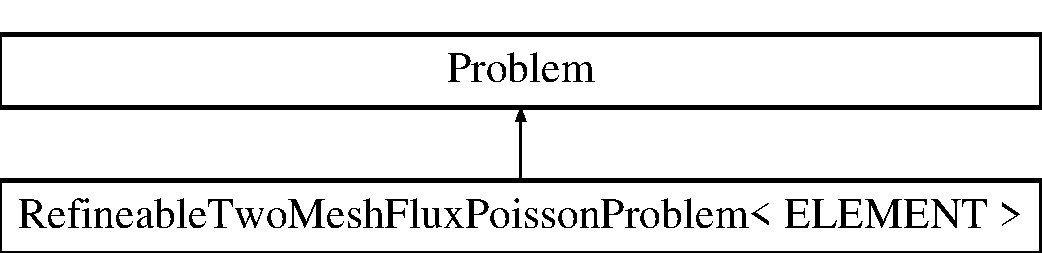
\includegraphics[height=2.000000cm]{classRefineableTwoMeshFluxPoissonProblem}
\end{center}
\end{figure}
\subsection*{Public Member Functions}
\begin{DoxyCompactItemize}
\item 
\hyperlink{classRefineableTwoMeshFluxPoissonProblem_a6568980564c4e39544b1c2bcb71cf3b6}{Refineable\+Two\+Mesh\+Flux\+Poisson\+Problem} (Poisson\+Equations$<$ 2 $>$\+::Poisson\+Source\+Fct\+Pt source\+\_\+fct\+\_\+pt)
\begin{DoxyCompactList}\small\item\em Constructor\+: Pass pointer to source function. \end{DoxyCompactList}\item 
\hyperlink{classRefineableTwoMeshFluxPoissonProblem_a6b1f154c77ea0c415bf171764d34302f}{$\sim$\+Refineable\+Two\+Mesh\+Flux\+Poisson\+Problem} ()
\begin{DoxyCompactList}\small\item\em Destructor (empty) \end{DoxyCompactList}\item 
void \hyperlink{classRefineableTwoMeshFluxPoissonProblem_ad9d4a3b5856839fa95f60968fabe3493}{doc\+\_\+solution} (Doc\+Info \&doc\+\_\+info)
\begin{DoxyCompactList}\small\item\em Doc the solution\+: doc\+\_\+info contains labels/output directory etc. \end{DoxyCompactList}\end{DoxyCompactItemize}
\subsection*{Private Member Functions}
\begin{DoxyCompactItemize}
\item 
void \hyperlink{classRefineableTwoMeshFluxPoissonProblem_a209506229c491a8cec4e1dce387e18c3}{actions\+\_\+before\+\_\+newton\+\_\+solve} ()
\begin{DoxyCompactList}\small\item\em Update the problem specs before solve\+: Reset boundary conditions to the values from the exact solution. \end{DoxyCompactList}\item 
void \hyperlink{classRefineableTwoMeshFluxPoissonProblem_ab8b04db3dab6297f609a9a028b1c4473}{actions\+\_\+after\+\_\+newton\+\_\+solve} ()
\begin{DoxyCompactList}\small\item\em Update the problem specs after solve (empty) \end{DoxyCompactList}\item 
void \hyperlink{classRefineableTwoMeshFluxPoissonProblem_a10d2a67a5ac599161ddcf876b31334f6}{actions\+\_\+before\+\_\+adapt} ()
\begin{DoxyCompactList}\small\item\em Actions before adapt\+: Wipe the mesh of prescribed flux elements. \end{DoxyCompactList}\item 
void \hyperlink{classRefineableTwoMeshFluxPoissonProblem_a0140155529861f5e63ab32feece3c9b6}{actions\+\_\+after\+\_\+adapt} ()
\begin{DoxyCompactList}\small\item\em Actions after adapt\+: Rebuild the mesh of prescribed flux elements. \end{DoxyCompactList}\item 
void \hyperlink{classRefineableTwoMeshFluxPoissonProblem_ac2eaf11cfc4dda41f97cacc2a1a1f86e}{create\+\_\+flux\+\_\+elements} (const unsigned \&b, Mesh $\ast$const \&bulk\+\_\+mesh\+\_\+pt, Mesh $\ast$const \&surface\+\_\+mesh\+\_\+pt)
\begin{DoxyCompactList}\small\item\em Create Poisson flux elements on boundary b of the Mesh pointed to by bulk\+\_\+mesh\+\_\+pt and add them to the Mesh object pointed to by surface\+\_\+mesh\+\_\+pt. \end{DoxyCompactList}\item 
void \hyperlink{classRefineableTwoMeshFluxPoissonProblem_ab35087cadc6dbc7a602441b9a986d650}{delete\+\_\+flux\+\_\+elements} (Mesh $\ast$const \&surface\+\_\+mesh\+\_\+pt)
\begin{DoxyCompactList}\small\item\em Delete Poisson flux elements and wipe the surface mesh. \end{DoxyCompactList}\item 
void \hyperlink{classRefineableTwoMeshFluxPoissonProblem_aa0aeec40bbdb0649e309e51ad96e5da7}{set\+\_\+prescribed\+\_\+flux\+\_\+pt} ()
\begin{DoxyCompactList}\small\item\em Set pointer to prescribed-\/flux function for all elements in the surface mesh. \end{DoxyCompactList}\end{DoxyCompactItemize}
\subsection*{Private Attributes}
\begin{DoxyCompactItemize}
\item 
\hyperlink{classSimpleRefineableRectangularQuadMesh}{Simple\+Refineable\+Rectangular\+Quad\+Mesh}$<$ E\+L\+E\+M\+E\+NT $>$ $\ast$ \hyperlink{classRefineableTwoMeshFluxPoissonProblem_a35746600caac7fd5b1a2ccec6beff8d6}{Bulk\+\_\+mesh\+\_\+pt}
\begin{DoxyCompactList}\small\item\em Pointer to the \char`\"{}bulk\char`\"{} mesh. \end{DoxyCompactList}\item 
Mesh $\ast$ \hyperlink{classRefineableTwoMeshFluxPoissonProblem_a1ad7c5a406b267f2d79c52b3d347971d}{Surface\+\_\+mesh\+\_\+pt}
\begin{DoxyCompactList}\small\item\em Pointer to the \char`\"{}surface\char`\"{} mesh. \end{DoxyCompactList}\item 
Poisson\+Equations$<$ 2 $>$\+::Poisson\+Source\+Fct\+Pt \hyperlink{classRefineableTwoMeshFluxPoissonProblem_a0f3434b437ca4b5e6a97ecae9e826477}{Source\+\_\+fct\+\_\+pt}
\begin{DoxyCompactList}\small\item\em Pointer to source function. \end{DoxyCompactList}\end{DoxyCompactItemize}


\subsection{Detailed Description}
\subsubsection*{template$<$class E\+L\+E\+M\+E\+NT$>$\newline
class Refineable\+Two\+Mesh\+Flux\+Poisson\+Problem$<$ E\+L\+E\+M\+E\+N\+T $>$}

2D Poisson problem on rectangular domain, discretised with 2D Q\+Poisson elements. Flux boundary conditions are applied along boundary 1 (the boundary where x=L). The specific type of element is specified via the template parameter. 

Definition at line 145 of file two\+\_\+d\+\_\+poisson\+\_\+flux\+\_\+bc\+\_\+adapt.\+cc.



\subsection{Constructor \& Destructor Documentation}
\mbox{\Hypertarget{classRefineableTwoMeshFluxPoissonProblem_a6568980564c4e39544b1c2bcb71cf3b6}\label{classRefineableTwoMeshFluxPoissonProblem_a6568980564c4e39544b1c2bcb71cf3b6}} 
\index{Refineable\+Two\+Mesh\+Flux\+Poisson\+Problem@{Refineable\+Two\+Mesh\+Flux\+Poisson\+Problem}!Refineable\+Two\+Mesh\+Flux\+Poisson\+Problem@{Refineable\+Two\+Mesh\+Flux\+Poisson\+Problem}}
\index{Refineable\+Two\+Mesh\+Flux\+Poisson\+Problem@{Refineable\+Two\+Mesh\+Flux\+Poisson\+Problem}!Refineable\+Two\+Mesh\+Flux\+Poisson\+Problem@{Refineable\+Two\+Mesh\+Flux\+Poisson\+Problem}}
\subsubsection{\texorpdfstring{Refineable\+Two\+Mesh\+Flux\+Poisson\+Problem()}{RefineableTwoMeshFluxPoissonProblem()}}
{\footnotesize\ttfamily template$<$class E\+L\+E\+M\+E\+NT $>$ \\
\hyperlink{classRefineableTwoMeshFluxPoissonProblem}{Refineable\+Two\+Mesh\+Flux\+Poisson\+Problem}$<$ E\+L\+E\+M\+E\+NT $>$\+::\hyperlink{classRefineableTwoMeshFluxPoissonProblem}{Refineable\+Two\+Mesh\+Flux\+Poisson\+Problem} (\begin{DoxyParamCaption}\item[{Poisson\+Equations$<$ 2 $>$\+::Poisson\+Source\+Fct\+Pt}]{source\+\_\+fct\+\_\+pt }\end{DoxyParamCaption})}



Constructor\+: Pass pointer to source function. 

Constructor for Poisson problem\+: Pass pointer to source function. 

Definition at line 208 of file two\+\_\+d\+\_\+poisson\+\_\+flux\+\_\+bc\+\_\+adapt.\+cc.



References Refineable\+Two\+Mesh\+Flux\+Poisson\+Problem$<$ E\+L\+E\+M\+E\+N\+T $>$\+::\+Bulk\+\_\+mesh\+\_\+pt, Refineable\+Two\+Mesh\+Flux\+Poisson\+Problem$<$ E\+L\+E\+M\+E\+N\+T $>$\+::create\+\_\+flux\+\_\+elements(), Refineable\+Two\+Mesh\+Flux\+Poisson\+Problem$<$ E\+L\+E\+M\+E\+N\+T $>$\+::set\+\_\+prescribed\+\_\+flux\+\_\+pt(), Refineable\+Two\+Mesh\+Flux\+Poisson\+Problem$<$ E\+L\+E\+M\+E\+N\+T $>$\+::\+Source\+\_\+fct\+\_\+pt, and Refineable\+Two\+Mesh\+Flux\+Poisson\+Problem$<$ E\+L\+E\+M\+E\+N\+T $>$\+::\+Surface\+\_\+mesh\+\_\+pt.

\mbox{\Hypertarget{classRefineableTwoMeshFluxPoissonProblem_a6b1f154c77ea0c415bf171764d34302f}\label{classRefineableTwoMeshFluxPoissonProblem_a6b1f154c77ea0c415bf171764d34302f}} 
\index{Refineable\+Two\+Mesh\+Flux\+Poisson\+Problem@{Refineable\+Two\+Mesh\+Flux\+Poisson\+Problem}!````~Refineable\+Two\+Mesh\+Flux\+Poisson\+Problem@{$\sim$\+Refineable\+Two\+Mesh\+Flux\+Poisson\+Problem}}
\index{````~Refineable\+Two\+Mesh\+Flux\+Poisson\+Problem@{$\sim$\+Refineable\+Two\+Mesh\+Flux\+Poisson\+Problem}!Refineable\+Two\+Mesh\+Flux\+Poisson\+Problem@{Refineable\+Two\+Mesh\+Flux\+Poisson\+Problem}}
\subsubsection{\texorpdfstring{$\sim$\+Refineable\+Two\+Mesh\+Flux\+Poisson\+Problem()}{~RefineableTwoMeshFluxPoissonProblem()}}
{\footnotesize\ttfamily template$<$class E\+L\+E\+M\+E\+NT$>$ \\
\hyperlink{classRefineableTwoMeshFluxPoissonProblem}{Refineable\+Two\+Mesh\+Flux\+Poisson\+Problem}$<$ E\+L\+E\+M\+E\+NT $>$\+::$\sim$\hyperlink{classRefineableTwoMeshFluxPoissonProblem}{Refineable\+Two\+Mesh\+Flux\+Poisson\+Problem} (\begin{DoxyParamCaption}{ }\end{DoxyParamCaption})\hspace{0.3cm}{\ttfamily [inline]}}



Destructor (empty) 



Definition at line 154 of file two\+\_\+d\+\_\+poisson\+\_\+flux\+\_\+bc\+\_\+adapt.\+cc.



\subsection{Member Function Documentation}
\mbox{\Hypertarget{classRefineableTwoMeshFluxPoissonProblem_a0140155529861f5e63ab32feece3c9b6}\label{classRefineableTwoMeshFluxPoissonProblem_a0140155529861f5e63ab32feece3c9b6}} 
\index{Refineable\+Two\+Mesh\+Flux\+Poisson\+Problem@{Refineable\+Two\+Mesh\+Flux\+Poisson\+Problem}!actions\+\_\+after\+\_\+adapt@{actions\+\_\+after\+\_\+adapt}}
\index{actions\+\_\+after\+\_\+adapt@{actions\+\_\+after\+\_\+adapt}!Refineable\+Two\+Mesh\+Flux\+Poisson\+Problem@{Refineable\+Two\+Mesh\+Flux\+Poisson\+Problem}}
\subsubsection{\texorpdfstring{actions\+\_\+after\+\_\+adapt()}{actions\_after\_adapt()}}
{\footnotesize\ttfamily template$<$class E\+L\+E\+M\+E\+NT $>$ \\
void \hyperlink{classRefineableTwoMeshFluxPoissonProblem}{Refineable\+Two\+Mesh\+Flux\+Poisson\+Problem}$<$ E\+L\+E\+M\+E\+NT $>$\+::actions\+\_\+after\+\_\+adapt (\begin{DoxyParamCaption}{ }\end{DoxyParamCaption})\hspace{0.3cm}{\ttfamily [private]}}



Actions after adapt\+: Rebuild the mesh of prescribed flux elements. 



Definition at line 358 of file two\+\_\+d\+\_\+poisson\+\_\+flux\+\_\+bc\+\_\+adapt.\+cc.



References Refineable\+Two\+Mesh\+Flux\+Poisson\+Problem$<$ E\+L\+E\+M\+E\+N\+T $>$\+::\+Bulk\+\_\+mesh\+\_\+pt, Refineable\+Two\+Mesh\+Flux\+Poisson\+Problem$<$ E\+L\+E\+M\+E\+N\+T $>$\+::create\+\_\+flux\+\_\+elements(), Refineable\+Two\+Mesh\+Flux\+Poisson\+Problem$<$ E\+L\+E\+M\+E\+N\+T $>$\+::set\+\_\+prescribed\+\_\+flux\+\_\+pt(), and Refineable\+Two\+Mesh\+Flux\+Poisson\+Problem$<$ E\+L\+E\+M\+E\+N\+T $>$\+::\+Surface\+\_\+mesh\+\_\+pt.

\mbox{\Hypertarget{classRefineableTwoMeshFluxPoissonProblem_ab8b04db3dab6297f609a9a028b1c4473}\label{classRefineableTwoMeshFluxPoissonProblem_ab8b04db3dab6297f609a9a028b1c4473}} 
\index{Refineable\+Two\+Mesh\+Flux\+Poisson\+Problem@{Refineable\+Two\+Mesh\+Flux\+Poisson\+Problem}!actions\+\_\+after\+\_\+newton\+\_\+solve@{actions\+\_\+after\+\_\+newton\+\_\+solve}}
\index{actions\+\_\+after\+\_\+newton\+\_\+solve@{actions\+\_\+after\+\_\+newton\+\_\+solve}!Refineable\+Two\+Mesh\+Flux\+Poisson\+Problem@{Refineable\+Two\+Mesh\+Flux\+Poisson\+Problem}}
\subsubsection{\texorpdfstring{actions\+\_\+after\+\_\+newton\+\_\+solve()}{actions\_after\_newton\_solve()}}
{\footnotesize\ttfamily template$<$class E\+L\+E\+M\+E\+NT$>$ \\
void \hyperlink{classRefineableTwoMeshFluxPoissonProblem}{Refineable\+Two\+Mesh\+Flux\+Poisson\+Problem}$<$ E\+L\+E\+M\+E\+NT $>$\+::actions\+\_\+after\+\_\+newton\+\_\+solve (\begin{DoxyParamCaption}{ }\end{DoxyParamCaption})\hspace{0.3cm}{\ttfamily [inline]}, {\ttfamily [private]}}



Update the problem specs after solve (empty) 



Definition at line 168 of file two\+\_\+d\+\_\+poisson\+\_\+flux\+\_\+bc\+\_\+adapt.\+cc.

\mbox{\Hypertarget{classRefineableTwoMeshFluxPoissonProblem_a10d2a67a5ac599161ddcf876b31334f6}\label{classRefineableTwoMeshFluxPoissonProblem_a10d2a67a5ac599161ddcf876b31334f6}} 
\index{Refineable\+Two\+Mesh\+Flux\+Poisson\+Problem@{Refineable\+Two\+Mesh\+Flux\+Poisson\+Problem}!actions\+\_\+before\+\_\+adapt@{actions\+\_\+before\+\_\+adapt}}
\index{actions\+\_\+before\+\_\+adapt@{actions\+\_\+before\+\_\+adapt}!Refineable\+Two\+Mesh\+Flux\+Poisson\+Problem@{Refineable\+Two\+Mesh\+Flux\+Poisson\+Problem}}
\subsubsection{\texorpdfstring{actions\+\_\+before\+\_\+adapt()}{actions\_before\_adapt()}}
{\footnotesize\ttfamily template$<$class E\+L\+E\+M\+E\+NT $>$ \\
void \hyperlink{classRefineableTwoMeshFluxPoissonProblem}{Refineable\+Two\+Mesh\+Flux\+Poisson\+Problem}$<$ E\+L\+E\+M\+E\+NT $>$\+::actions\+\_\+before\+\_\+adapt (\begin{DoxyParamCaption}{ }\end{DoxyParamCaption})\hspace{0.3cm}{\ttfamily [private]}}



Actions before adapt\+: Wipe the mesh of prescribed flux elements. 



Definition at line 342 of file two\+\_\+d\+\_\+poisson\+\_\+flux\+\_\+bc\+\_\+adapt.\+cc.



References Refineable\+Two\+Mesh\+Flux\+Poisson\+Problem$<$ E\+L\+E\+M\+E\+N\+T $>$\+::delete\+\_\+flux\+\_\+elements(), and Refineable\+Two\+Mesh\+Flux\+Poisson\+Problem$<$ E\+L\+E\+M\+E\+N\+T $>$\+::\+Surface\+\_\+mesh\+\_\+pt.

\mbox{\Hypertarget{classRefineableTwoMeshFluxPoissonProblem_a209506229c491a8cec4e1dce387e18c3}\label{classRefineableTwoMeshFluxPoissonProblem_a209506229c491a8cec4e1dce387e18c3}} 
\index{Refineable\+Two\+Mesh\+Flux\+Poisson\+Problem@{Refineable\+Two\+Mesh\+Flux\+Poisson\+Problem}!actions\+\_\+before\+\_\+newton\+\_\+solve@{actions\+\_\+before\+\_\+newton\+\_\+solve}}
\index{actions\+\_\+before\+\_\+newton\+\_\+solve@{actions\+\_\+before\+\_\+newton\+\_\+solve}!Refineable\+Two\+Mesh\+Flux\+Poisson\+Problem@{Refineable\+Two\+Mesh\+Flux\+Poisson\+Problem}}
\subsubsection{\texorpdfstring{actions\+\_\+before\+\_\+newton\+\_\+solve()}{actions\_before\_newton\_solve()}}
{\footnotesize\ttfamily template$<$class E\+L\+E\+M\+E\+NT $>$ \\
void \hyperlink{classRefineableTwoMeshFluxPoissonProblem}{Refineable\+Two\+Mesh\+Flux\+Poisson\+Problem}$<$ E\+L\+E\+M\+E\+NT $>$\+::actions\+\_\+before\+\_\+newton\+\_\+solve (\begin{DoxyParamCaption}{ }\end{DoxyParamCaption})\hspace{0.3cm}{\ttfamily [private]}}



Update the problem specs before solve\+: Reset boundary conditions to the values from the exact solution. 

Update the problem specs before solve\+: Reset boundary conditions to the values from the exact solution. 

Definition at line 300 of file two\+\_\+d\+\_\+poisson\+\_\+flux\+\_\+bc\+\_\+adapt.\+cc.



References Refineable\+Two\+Mesh\+Flux\+Poisson\+Problem$<$ E\+L\+E\+M\+E\+N\+T $>$\+::\+Bulk\+\_\+mesh\+\_\+pt, and Tanh\+Soln\+For\+Poisson\+::get\+\_\+exact\+\_\+u().

\mbox{\Hypertarget{classRefineableTwoMeshFluxPoissonProblem_ac2eaf11cfc4dda41f97cacc2a1a1f86e}\label{classRefineableTwoMeshFluxPoissonProblem_ac2eaf11cfc4dda41f97cacc2a1a1f86e}} 
\index{Refineable\+Two\+Mesh\+Flux\+Poisson\+Problem@{Refineable\+Two\+Mesh\+Flux\+Poisson\+Problem}!create\+\_\+flux\+\_\+elements@{create\+\_\+flux\+\_\+elements}}
\index{create\+\_\+flux\+\_\+elements@{create\+\_\+flux\+\_\+elements}!Refineable\+Two\+Mesh\+Flux\+Poisson\+Problem@{Refineable\+Two\+Mesh\+Flux\+Poisson\+Problem}}
\subsubsection{\texorpdfstring{create\+\_\+flux\+\_\+elements()}{create\_flux\_elements()}}
{\footnotesize\ttfamily template$<$class E\+L\+E\+M\+E\+NT $>$ \\
void \hyperlink{classRefineableTwoMeshFluxPoissonProblem}{Refineable\+Two\+Mesh\+Flux\+Poisson\+Problem}$<$ E\+L\+E\+M\+E\+NT $>$\+::create\+\_\+flux\+\_\+elements (\begin{DoxyParamCaption}\item[{const unsigned \&}]{b,  }\item[{Mesh $\ast$const \&}]{bulk\+\_\+mesh\+\_\+pt,  }\item[{Mesh $\ast$const \&}]{surface\+\_\+mesh\+\_\+pt }\end{DoxyParamCaption})\hspace{0.3cm}{\ttfamily [private]}}



Create Poisson flux elements on boundary b of the Mesh pointed to by bulk\+\_\+mesh\+\_\+pt and add them to the Mesh object pointed to by surface\+\_\+mesh\+\_\+pt. 

Create Poisson Flux Elements on the b-\/th boundary of the Mesh object pointed to by bulk\+\_\+mesh\+\_\+pt and add the elements to the Mesh object pointeed to by surface\+\_\+mesh\+\_\+pt. 

Definition at line 475 of file two\+\_\+d\+\_\+poisson\+\_\+flux\+\_\+bc\+\_\+adapt.\+cc.



References Refineable\+Two\+Mesh\+Flux\+Poisson\+Problem$<$ E\+L\+E\+M\+E\+N\+T $>$\+::delete\+\_\+flux\+\_\+elements().



Referenced by Refineable\+Two\+Mesh\+Flux\+Poisson\+Problem$<$ E\+L\+E\+M\+E\+N\+T $>$\+::actions\+\_\+after\+\_\+adapt(), Refineable\+Two\+Mesh\+Flux\+Poisson\+Problem$<$ E\+L\+E\+M\+E\+N\+T $>$\+::doc\+\_\+solution(), and Refineable\+Two\+Mesh\+Flux\+Poisson\+Problem$<$ E\+L\+E\+M\+E\+N\+T $>$\+::\+Refineable\+Two\+Mesh\+Flux\+Poisson\+Problem().

\mbox{\Hypertarget{classRefineableTwoMeshFluxPoissonProblem_ab35087cadc6dbc7a602441b9a986d650}\label{classRefineableTwoMeshFluxPoissonProblem_ab35087cadc6dbc7a602441b9a986d650}} 
\index{Refineable\+Two\+Mesh\+Flux\+Poisson\+Problem@{Refineable\+Two\+Mesh\+Flux\+Poisson\+Problem}!delete\+\_\+flux\+\_\+elements@{delete\+\_\+flux\+\_\+elements}}
\index{delete\+\_\+flux\+\_\+elements@{delete\+\_\+flux\+\_\+elements}!Refineable\+Two\+Mesh\+Flux\+Poisson\+Problem@{Refineable\+Two\+Mesh\+Flux\+Poisson\+Problem}}
\subsubsection{\texorpdfstring{delete\+\_\+flux\+\_\+elements()}{delete\_flux\_elements()}}
{\footnotesize\ttfamily template$<$class E\+L\+E\+M\+E\+NT $>$ \\
void \hyperlink{classRefineableTwoMeshFluxPoissonProblem}{Refineable\+Two\+Mesh\+Flux\+Poisson\+Problem}$<$ E\+L\+E\+M\+E\+NT $>$\+::delete\+\_\+flux\+\_\+elements (\begin{DoxyParamCaption}\item[{Mesh $\ast$const \&}]{surface\+\_\+mesh\+\_\+pt }\end{DoxyParamCaption})\hspace{0.3cm}{\ttfamily [private]}}



Delete Poisson flux elements and wipe the surface mesh. 

Delete Poisson Flux Elements and wipe the surface mesh. 

Definition at line 509 of file two\+\_\+d\+\_\+poisson\+\_\+flux\+\_\+bc\+\_\+adapt.\+cc.



Referenced by Refineable\+Two\+Mesh\+Flux\+Poisson\+Problem$<$ E\+L\+E\+M\+E\+N\+T $>$\+::actions\+\_\+before\+\_\+adapt(), and Refineable\+Two\+Mesh\+Flux\+Poisson\+Problem$<$ E\+L\+E\+M\+E\+N\+T $>$\+::create\+\_\+flux\+\_\+elements().

\mbox{\Hypertarget{classRefineableTwoMeshFluxPoissonProblem_ad9d4a3b5856839fa95f60968fabe3493}\label{classRefineableTwoMeshFluxPoissonProblem_ad9d4a3b5856839fa95f60968fabe3493}} 
\index{Refineable\+Two\+Mesh\+Flux\+Poisson\+Problem@{Refineable\+Two\+Mesh\+Flux\+Poisson\+Problem}!doc\+\_\+solution@{doc\+\_\+solution}}
\index{doc\+\_\+solution@{doc\+\_\+solution}!Refineable\+Two\+Mesh\+Flux\+Poisson\+Problem@{Refineable\+Two\+Mesh\+Flux\+Poisson\+Problem}}
\subsubsection{\texorpdfstring{doc\+\_\+solution()}{doc\_solution()}}
{\footnotesize\ttfamily template$<$class E\+L\+E\+M\+E\+NT $>$ \\
void \hyperlink{classRefineableTwoMeshFluxPoissonProblem}{Refineable\+Two\+Mesh\+Flux\+Poisson\+Problem}$<$ E\+L\+E\+M\+E\+NT $>$\+::doc\+\_\+solution (\begin{DoxyParamCaption}\item[{Doc\+Info \&}]{doc\+\_\+info }\end{DoxyParamCaption})}



Doc the solution\+: doc\+\_\+info contains labels/output directory etc. 

Doc the solution. Doc\+Info object stores flags/labels for where the output gets written to 

Definition at line 413 of file two\+\_\+d\+\_\+poisson\+\_\+flux\+\_\+bc\+\_\+adapt.\+cc.



References Refineable\+Two\+Mesh\+Flux\+Poisson\+Problem$<$ E\+L\+E\+M\+E\+N\+T $>$\+::\+Bulk\+\_\+mesh\+\_\+pt, Refineable\+Two\+Mesh\+Flux\+Poisson\+Problem$<$ E\+L\+E\+M\+E\+N\+T $>$\+::create\+\_\+flux\+\_\+elements(), and Tanh\+Soln\+For\+Poisson\+::get\+\_\+exact\+\_\+u().



Referenced by main().

\mbox{\Hypertarget{classRefineableTwoMeshFluxPoissonProblem_aa0aeec40bbdb0649e309e51ad96e5da7}\label{classRefineableTwoMeshFluxPoissonProblem_aa0aeec40bbdb0649e309e51ad96e5da7}} 
\index{Refineable\+Two\+Mesh\+Flux\+Poisson\+Problem@{Refineable\+Two\+Mesh\+Flux\+Poisson\+Problem}!set\+\_\+prescribed\+\_\+flux\+\_\+pt@{set\+\_\+prescribed\+\_\+flux\+\_\+pt}}
\index{set\+\_\+prescribed\+\_\+flux\+\_\+pt@{set\+\_\+prescribed\+\_\+flux\+\_\+pt}!Refineable\+Two\+Mesh\+Flux\+Poisson\+Problem@{Refineable\+Two\+Mesh\+Flux\+Poisson\+Problem}}
\subsubsection{\texorpdfstring{set\+\_\+prescribed\+\_\+flux\+\_\+pt()}{set\_prescribed\_flux\_pt()}}
{\footnotesize\ttfamily template$<$class E\+L\+E\+M\+E\+NT $>$ \\
void \hyperlink{classRefineableTwoMeshFluxPoissonProblem}{Refineable\+Two\+Mesh\+Flux\+Poisson\+Problem}$<$ E\+L\+E\+M\+E\+NT $>$\+::set\+\_\+prescribed\+\_\+flux\+\_\+pt (\begin{DoxyParamCaption}{ }\end{DoxyParamCaption})\hspace{0.3cm}{\ttfamily [private]}}



Set pointer to prescribed-\/flux function for all elements in the surface mesh. 

Set pointer to prescribed-\/flux function for all elements in the surface mesh 

Definition at line 388 of file two\+\_\+d\+\_\+poisson\+\_\+flux\+\_\+bc\+\_\+adapt.\+cc.



References Tanh\+Soln\+For\+Poisson\+::prescribed\+\_\+flux\+\_\+on\+\_\+fixed\+\_\+x\+\_\+boundary(), and Refineable\+Two\+Mesh\+Flux\+Poisson\+Problem$<$ E\+L\+E\+M\+E\+N\+T $>$\+::\+Surface\+\_\+mesh\+\_\+pt.



Referenced by Refineable\+Two\+Mesh\+Flux\+Poisson\+Problem$<$ E\+L\+E\+M\+E\+N\+T $>$\+::actions\+\_\+after\+\_\+adapt(), and Refineable\+Two\+Mesh\+Flux\+Poisson\+Problem$<$ E\+L\+E\+M\+E\+N\+T $>$\+::\+Refineable\+Two\+Mesh\+Flux\+Poisson\+Problem().



\subsection{Member Data Documentation}
\mbox{\Hypertarget{classRefineableTwoMeshFluxPoissonProblem_a35746600caac7fd5b1a2ccec6beff8d6}\label{classRefineableTwoMeshFluxPoissonProblem_a35746600caac7fd5b1a2ccec6beff8d6}} 
\index{Refineable\+Two\+Mesh\+Flux\+Poisson\+Problem@{Refineable\+Two\+Mesh\+Flux\+Poisson\+Problem}!Bulk\+\_\+mesh\+\_\+pt@{Bulk\+\_\+mesh\+\_\+pt}}
\index{Bulk\+\_\+mesh\+\_\+pt@{Bulk\+\_\+mesh\+\_\+pt}!Refineable\+Two\+Mesh\+Flux\+Poisson\+Problem@{Refineable\+Two\+Mesh\+Flux\+Poisson\+Problem}}
\subsubsection{\texorpdfstring{Bulk\+\_\+mesh\+\_\+pt}{Bulk\_mesh\_pt}}
{\footnotesize\ttfamily template$<$class E\+L\+E\+M\+E\+NT$>$ \\
\hyperlink{classSimpleRefineableRectangularQuadMesh}{Simple\+Refineable\+Rectangular\+Quad\+Mesh}$<$E\+L\+E\+M\+E\+NT$>$$\ast$ \hyperlink{classRefineableTwoMeshFluxPoissonProblem}{Refineable\+Two\+Mesh\+Flux\+Poisson\+Problem}$<$ E\+L\+E\+M\+E\+NT $>$\+::Bulk\+\_\+mesh\+\_\+pt\hspace{0.3cm}{\ttfamily [private]}}



Pointer to the \char`\"{}bulk\char`\"{} mesh. 



Definition at line 190 of file two\+\_\+d\+\_\+poisson\+\_\+flux\+\_\+bc\+\_\+adapt.\+cc.



Referenced by Refineable\+Two\+Mesh\+Flux\+Poisson\+Problem$<$ E\+L\+E\+M\+E\+N\+T $>$\+::actions\+\_\+after\+\_\+adapt(), Refineable\+Two\+Mesh\+Flux\+Poisson\+Problem$<$ E\+L\+E\+M\+E\+N\+T $>$\+::actions\+\_\+before\+\_\+newton\+\_\+solve(), Refineable\+Two\+Mesh\+Flux\+Poisson\+Problem$<$ E\+L\+E\+M\+E\+N\+T $>$\+::doc\+\_\+solution(), and Refineable\+Two\+Mesh\+Flux\+Poisson\+Problem$<$ E\+L\+E\+M\+E\+N\+T $>$\+::\+Refineable\+Two\+Mesh\+Flux\+Poisson\+Problem().

\mbox{\Hypertarget{classRefineableTwoMeshFluxPoissonProblem_a0f3434b437ca4b5e6a97ecae9e826477}\label{classRefineableTwoMeshFluxPoissonProblem_a0f3434b437ca4b5e6a97ecae9e826477}} 
\index{Refineable\+Two\+Mesh\+Flux\+Poisson\+Problem@{Refineable\+Two\+Mesh\+Flux\+Poisson\+Problem}!Source\+\_\+fct\+\_\+pt@{Source\+\_\+fct\+\_\+pt}}
\index{Source\+\_\+fct\+\_\+pt@{Source\+\_\+fct\+\_\+pt}!Refineable\+Two\+Mesh\+Flux\+Poisson\+Problem@{Refineable\+Two\+Mesh\+Flux\+Poisson\+Problem}}
\subsubsection{\texorpdfstring{Source\+\_\+fct\+\_\+pt}{Source\_fct\_pt}}
{\footnotesize\ttfamily template$<$class E\+L\+E\+M\+E\+NT$>$ \\
Poisson\+Equations$<$2$>$\+::Poisson\+Source\+Fct\+Pt \hyperlink{classRefineableTwoMeshFluxPoissonProblem}{Refineable\+Two\+Mesh\+Flux\+Poisson\+Problem}$<$ E\+L\+E\+M\+E\+NT $>$\+::Source\+\_\+fct\+\_\+pt\hspace{0.3cm}{\ttfamily [private]}}



Pointer to source function. 



Definition at line 196 of file two\+\_\+d\+\_\+poisson\+\_\+flux\+\_\+bc\+\_\+adapt.\+cc.



Referenced by Refineable\+Two\+Mesh\+Flux\+Poisson\+Problem$<$ E\+L\+E\+M\+E\+N\+T $>$\+::\+Refineable\+Two\+Mesh\+Flux\+Poisson\+Problem().

\mbox{\Hypertarget{classRefineableTwoMeshFluxPoissonProblem_a1ad7c5a406b267f2d79c52b3d347971d}\label{classRefineableTwoMeshFluxPoissonProblem_a1ad7c5a406b267f2d79c52b3d347971d}} 
\index{Refineable\+Two\+Mesh\+Flux\+Poisson\+Problem@{Refineable\+Two\+Mesh\+Flux\+Poisson\+Problem}!Surface\+\_\+mesh\+\_\+pt@{Surface\+\_\+mesh\+\_\+pt}}
\index{Surface\+\_\+mesh\+\_\+pt@{Surface\+\_\+mesh\+\_\+pt}!Refineable\+Two\+Mesh\+Flux\+Poisson\+Problem@{Refineable\+Two\+Mesh\+Flux\+Poisson\+Problem}}
\subsubsection{\texorpdfstring{Surface\+\_\+mesh\+\_\+pt}{Surface\_mesh\_pt}}
{\footnotesize\ttfamily template$<$class E\+L\+E\+M\+E\+NT$>$ \\
Mesh$\ast$ \hyperlink{classRefineableTwoMeshFluxPoissonProblem}{Refineable\+Two\+Mesh\+Flux\+Poisson\+Problem}$<$ E\+L\+E\+M\+E\+NT $>$\+::Surface\+\_\+mesh\+\_\+pt\hspace{0.3cm}{\ttfamily [private]}}



Pointer to the \char`\"{}surface\char`\"{} mesh. 



Definition at line 193 of file two\+\_\+d\+\_\+poisson\+\_\+flux\+\_\+bc\+\_\+adapt.\+cc.



Referenced by Refineable\+Two\+Mesh\+Flux\+Poisson\+Problem$<$ E\+L\+E\+M\+E\+N\+T $>$\+::actions\+\_\+after\+\_\+adapt(), Refineable\+Two\+Mesh\+Flux\+Poisson\+Problem$<$ E\+L\+E\+M\+E\+N\+T $>$\+::actions\+\_\+before\+\_\+adapt(), Refineable\+Two\+Mesh\+Flux\+Poisson\+Problem$<$ E\+L\+E\+M\+E\+N\+T $>$\+::\+Refineable\+Two\+Mesh\+Flux\+Poisson\+Problem(), and Refineable\+Two\+Mesh\+Flux\+Poisson\+Problem$<$ E\+L\+E\+M\+E\+N\+T $>$\+::set\+\_\+prescribed\+\_\+flux\+\_\+pt().



The documentation for this class was generated from the following file\+:\begin{DoxyCompactItemize}
\item 
\hyperlink{two__d__poisson__flux__bc__adapt_8cc}{two\+\_\+d\+\_\+poisson\+\_\+flux\+\_\+bc\+\_\+adapt.\+cc}\end{DoxyCompactItemize}

\hypertarget{classSimpleRefineableRectangularQuadMesh}{}\section{Simple\+Refineable\+Rectangular\+Quad\+Mesh$<$ E\+L\+E\+M\+E\+NT $>$ Class Template Reference}
\label{classSimpleRefineableRectangularQuadMesh}\index{Simple\+Refineable\+Rectangular\+Quad\+Mesh$<$ E\+L\+E\+M\+E\+N\+T $>$@{Simple\+Refineable\+Rectangular\+Quad\+Mesh$<$ E\+L\+E\+M\+E\+N\+T $>$}}
Inheritance diagram for Simple\+Refineable\+Rectangular\+Quad\+Mesh$<$ E\+L\+E\+M\+E\+NT $>$\+:\begin{figure}[H]
\begin{center}
\leavevmode
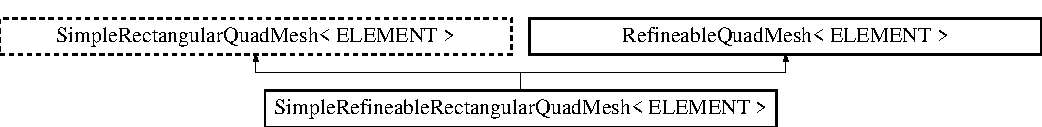
\includegraphics[height=1.702128cm]{classSimpleRefineableRectangularQuadMesh}
\end{center}
\end{figure}
\subsection*{Public Member Functions}
\begin{DoxyCompactItemize}
\item 
\hyperlink{classSimpleRefineableRectangularQuadMesh_ae0eab85a2c97fce00d7c82a613378e79}{Simple\+Refineable\+Rectangular\+Quad\+Mesh} (const unsigned \&Nx, const unsigned \&Ny, const double \&Lx, const double \&Ly, Time\+Stepper $\ast$time\+\_\+stepper\+\_\+pt=\&Mesh\+::\+Default\+\_\+\+Time\+Stepper)
\begin{DoxyCompactList}\small\item\em Pass number of elements in the horizontal and vertical directions, and the corresponding dimensions. Timestepper defaults to Static. \end{DoxyCompactList}\item 
virtual \hyperlink{classSimpleRefineableRectangularQuadMesh_a8f258e0b5178ccb33f0596ae5a33c3c5}{$\sim$\+Simple\+Refineable\+Rectangular\+Quad\+Mesh} ()
\begin{DoxyCompactList}\small\item\em Destructor\+: Empty. \end{DoxyCompactList}\end{DoxyCompactItemize}


\subsection{Detailed Description}
\subsubsection*{template$<$class E\+L\+E\+M\+E\+NT$>$\newline
class Simple\+Refineable\+Rectangular\+Quad\+Mesh$<$ E\+L\+E\+M\+E\+N\+T $>$}

Refineable equivalent of the Simple\+Rectangular\+Quad\+Mesh. Refinement is performed by the Quad\+Tree-\/based procedures implemented in the Refineable\+Quad\+Mesh base class. 

Definition at line 56 of file two\+\_\+d\+\_\+poisson\+\_\+adapt.\+cc.



\subsection{Constructor \& Destructor Documentation}
\mbox{\Hypertarget{classSimpleRefineableRectangularQuadMesh_ae0eab85a2c97fce00d7c82a613378e79}\label{classSimpleRefineableRectangularQuadMesh_ae0eab85a2c97fce00d7c82a613378e79}} 
\index{Simple\+Refineable\+Rectangular\+Quad\+Mesh@{Simple\+Refineable\+Rectangular\+Quad\+Mesh}!Simple\+Refineable\+Rectangular\+Quad\+Mesh@{Simple\+Refineable\+Rectangular\+Quad\+Mesh}}
\index{Simple\+Refineable\+Rectangular\+Quad\+Mesh@{Simple\+Refineable\+Rectangular\+Quad\+Mesh}!Simple\+Refineable\+Rectangular\+Quad\+Mesh@{Simple\+Refineable\+Rectangular\+Quad\+Mesh}}
\subsubsection{\texorpdfstring{Simple\+Refineable\+Rectangular\+Quad\+Mesh()}{SimpleRefineableRectangularQuadMesh()}}
{\footnotesize\ttfamily template$<$class E\+L\+E\+M\+E\+NT$>$ \\
\hyperlink{classSimpleRefineableRectangularQuadMesh}{Simple\+Refineable\+Rectangular\+Quad\+Mesh}$<$ E\+L\+E\+M\+E\+NT $>$\+::\hyperlink{classSimpleRefineableRectangularQuadMesh}{Simple\+Refineable\+Rectangular\+Quad\+Mesh} (\begin{DoxyParamCaption}\item[{const unsigned \&}]{Nx,  }\item[{const unsigned \&}]{Ny,  }\item[{const double \&}]{Lx,  }\item[{const double \&}]{Ly,  }\item[{Time\+Stepper $\ast$}]{time\+\_\+stepper\+\_\+pt = {\ttfamily \&Mesh\+:\+:Default\+\_\+TimeStepper} }\end{DoxyParamCaption})\hspace{0.3cm}{\ttfamily [inline]}}



Pass number of elements in the horizontal and vertical directions, and the corresponding dimensions. Timestepper defaults to Static. 



Definition at line 66 of file two\+\_\+d\+\_\+poisson\+\_\+adapt.\+cc.

\mbox{\Hypertarget{classSimpleRefineableRectangularQuadMesh_a8f258e0b5178ccb33f0596ae5a33c3c5}\label{classSimpleRefineableRectangularQuadMesh_a8f258e0b5178ccb33f0596ae5a33c3c5}} 
\index{Simple\+Refineable\+Rectangular\+Quad\+Mesh@{Simple\+Refineable\+Rectangular\+Quad\+Mesh}!````~Simple\+Refineable\+Rectangular\+Quad\+Mesh@{$\sim$\+Simple\+Refineable\+Rectangular\+Quad\+Mesh}}
\index{````~Simple\+Refineable\+Rectangular\+Quad\+Mesh@{$\sim$\+Simple\+Refineable\+Rectangular\+Quad\+Mesh}!Simple\+Refineable\+Rectangular\+Quad\+Mesh@{Simple\+Refineable\+Rectangular\+Quad\+Mesh}}
\subsubsection{\texorpdfstring{$\sim$\+Simple\+Refineable\+Rectangular\+Quad\+Mesh()}{~SimpleRefineableRectangularQuadMesh()}}
{\footnotesize\ttfamily template$<$class E\+L\+E\+M\+E\+NT$>$ \\
virtual \hyperlink{classSimpleRefineableRectangularQuadMesh}{Simple\+Refineable\+Rectangular\+Quad\+Mesh}$<$ E\+L\+E\+M\+E\+NT $>$\+::$\sim$\hyperlink{classSimpleRefineableRectangularQuadMesh}{Simple\+Refineable\+Rectangular\+Quad\+Mesh} (\begin{DoxyParamCaption}{ }\end{DoxyParamCaption})\hspace{0.3cm}{\ttfamily [inline]}, {\ttfamily [virtual]}}



Destructor\+: Empty. 



Definition at line 83 of file two\+\_\+d\+\_\+poisson\+\_\+adapt.\+cc.



The documentation for this class was generated from the following file\+:\begin{DoxyCompactItemize}
\item 
\hyperlink{two__d__poisson__adapt_8cc}{two\+\_\+d\+\_\+poisson\+\_\+adapt.\+cc}\end{DoxyCompactItemize}

\chapter{File Documentation}
\hypertarget{two__d__poisson__flux__bc__adapt_8cc}{}\section{two\+\_\+d\+\_\+poisson\+\_\+flux\+\_\+bc\+\_\+adapt.\+cc File Reference}
\label{two__d__poisson__flux__bc__adapt_8cc}\index{two\+\_\+d\+\_\+poisson\+\_\+flux\+\_\+bc\+\_\+adapt.\+cc@{two\+\_\+d\+\_\+poisson\+\_\+flux\+\_\+bc\+\_\+adapt.\+cc}}
\subsection*{Classes}
\begin{DoxyCompactItemize}
\item 
class \hyperlink{classSimpleRefineableRectangularQuadMesh}{Simple\+Refineable\+Rectangular\+Quad\+Mesh$<$ E\+L\+E\+M\+E\+N\+T $>$}
\item 
class \hyperlink{classRefineableTwoMeshFluxPoissonProblem}{Refineable\+Two\+Mesh\+Flux\+Poisson\+Problem$<$ E\+L\+E\+M\+E\+N\+T $>$}
\end{DoxyCompactItemize}
\subsection*{Namespaces}
\begin{DoxyCompactItemize}
\item 
 \hyperlink{namespaceTanhSolnForPoisson}{Tanh\+Soln\+For\+Poisson}
\begin{DoxyCompactList}\small\item\em Namespace for exact solution for Poisson equation with \char`\"{}sharp step\char`\"{}. \end{DoxyCompactList}\end{DoxyCompactItemize}
\subsection*{Functions}
\begin{DoxyCompactItemize}
\item 
void \hyperlink{namespaceTanhSolnForPoisson_af7896e9c18ce6438c73ae2a875e8b7de}{Tanh\+Soln\+For\+Poisson\+::get\+\_\+exact\+\_\+u} (const Vector$<$ double $>$ \&x, Vector$<$ double $>$ \&u)
\begin{DoxyCompactList}\small\item\em Exact solution as a Vector. \end{DoxyCompactList}\item 
void \hyperlink{namespaceTanhSolnForPoisson_a967bc28320e02534beb714846b63e251}{Tanh\+Soln\+For\+Poisson\+::source\+\_\+function} (const Vector$<$ double $>$ \&x, double \&source)
\begin{DoxyCompactList}\small\item\em Source function required to make the solution above an exact solution. \end{DoxyCompactList}\item 
void \hyperlink{namespaceTanhSolnForPoisson_a0e99ccf27df36f28f091de6d57484172}{Tanh\+Soln\+For\+Poisson\+::prescribed\+\_\+flux\+\_\+on\+\_\+fixed\+\_\+x\+\_\+boundary} (const Vector$<$ double $>$ \&x, double \&flux)
\begin{DoxyCompactList}\small\item\em Flux required by the exact solution on a boundary on which x is fixed. \end{DoxyCompactList}\item 
int \hyperlink{two__d__poisson__flux__bc__adapt_8cc_ae66f6b31b5ad750f1fe042a706a4e3d4}{main} ()
\end{DoxyCompactItemize}
\subsection*{Variables}
\begin{DoxyCompactItemize}
\item 
double \hyperlink{namespaceTanhSolnForPoisson_ae676ccd186d5df119cce811596d949c1}{Tanh\+Soln\+For\+Poisson\+::\+Alpha} =1.\+0
\begin{DoxyCompactList}\small\item\em Parameter for steepness of \char`\"{}step\char`\"{}. \end{DoxyCompactList}\item 
double \hyperlink{namespaceTanhSolnForPoisson_a785ccd00a727125a5138fbbcac173294}{Tanh\+Soln\+For\+Poisson\+::\+Tan\+Phi} =0.\+0
\begin{DoxyCompactList}\small\item\em Parameter for angle Phi of \char`\"{}step\char`\"{}. \end{DoxyCompactList}\end{DoxyCompactItemize}


\subsection{Function Documentation}
\mbox{\Hypertarget{two__d__poisson__flux__bc__adapt_8cc_ae66f6b31b5ad750f1fe042a706a4e3d4}\label{two__d__poisson__flux__bc__adapt_8cc_ae66f6b31b5ad750f1fe042a706a4e3d4}} 
\index{two\+\_\+d\+\_\+poisson\+\_\+flux\+\_\+bc\+\_\+adapt.\+cc@{two\+\_\+d\+\_\+poisson\+\_\+flux\+\_\+bc\+\_\+adapt.\+cc}!main@{main}}
\index{main@{main}!two\+\_\+d\+\_\+poisson\+\_\+flux\+\_\+bc\+\_\+adapt.\+cc@{two\+\_\+d\+\_\+poisson\+\_\+flux\+\_\+bc\+\_\+adapt.\+cc}}
\subsubsection{\texorpdfstring{main()}{main()}}
{\footnotesize\ttfamily int main (\begin{DoxyParamCaption}{ }\end{DoxyParamCaption})}

Demonstrate how to solve 2D Poisson problem with flux boundary conditions, using two meshes. 

Definition at line 532 of file two\+\_\+d\+\_\+poisson\+\_\+flux\+\_\+bc\+\_\+adapt.\+cc.



References Tanh\+Soln\+For\+Poisson\+::\+Alpha, Refineable\+Two\+Mesh\+Flux\+Poisson\+Problem$<$ E\+L\+E\+M\+E\+N\+T $>$\+::doc\+\_\+solution(), Tanh\+Soln\+For\+Poisson\+::source\+\_\+function(), and Tanh\+Soln\+For\+Poisson\+::\+Tan\+Phi.


\hypertarget{two__d__poisson__flux__bc__adapt_8txt__doxygenified_8h}{}\section{two\+\_\+d\+\_\+poisson\+\_\+flux\+\_\+bc\+\_\+adapt.\+txt\+\_\+doxygenified.\+h File Reference}
\label{two__d__poisson__flux__bc__adapt_8txt__doxygenified_8h}\index{two\+\_\+d\+\_\+poisson\+\_\+flux\+\_\+bc\+\_\+adapt.\+txt\+\_\+doxygenified.\+h@{two\+\_\+d\+\_\+poisson\+\_\+flux\+\_\+bc\+\_\+adapt.\+txt\+\_\+doxygenified.\+h}}

%--- End generated contents ---

% Index
\backmatter
\newpage
\phantomsection
\clearemptydoublepage
\addcontentsline{toc}{chapter}{Index}
\printindex

\end{document}
